\section{Fermion Halo and Dark Matter in the Galaxy}
\begin{quotation}
	\raggedleft \it I believe there are
	15,747,724,136,275,002,577,605,653,961,181,555,468,044,\\
	717,914,527,116,709,366,231,425,076,185,631,031,296 \\
	protons in the universe and the same number of electrons.\\
	-- Sir Arthur Eddington
\end{quotation}
An extension of the fermion ball theory is to consider fermions with finite temperature \cite{ref_finitetemp}.
Such an extension results in a fermion halo around
the central ball already investigated in this thesis. In this section, we briefly discuss how the finite temperature extension leads to a
halo structure and the effect this has upon the dark matter problem in our galaxy \cite{ref_halo}.

\subsection{Dark Matter Within Our Galaxy}
It is well known, from the rotation curves of an increasing number of galaxies, that there are substantial amounts of dark matter in the halos
of galaxies. Typically, dark matter contributes about 10 times more mass than the ordinary matter which is contained in visible stars, dust
and gas. It is worthwhile to speculate that the super-massive compact dark objects at the galactic centres may have something to do with the
dark matter in the halos.

In the case of the Milky Way, this dark matter is arranged in a nearly spherically symmetric halo, stretching roughly a third the distance to
the Andromeda galaxy in radial component. There are a number of indications from nucleosynthesis \cite{ref_halonucleo},
micro-lensing \cite{ref_halomicrolens}, structure formation and microwave background data \cite{ref_halocmbstruct},
which indicates at least part of this dark matter halo cannot be made of ordinary matter. In the following, we will be primarily
concerned with this non-baryonic dark matter which does not interact efficiently with ordinary matter and radiation, except gravitationally.

Cold dark matter scenarios provide an excellent description of the formation of the large-scale structure in the universe. However, they fail
on galactic and sub-galactic scales \cite{ref_halofailcdm} because the absence of velocity dispersion causes the dark matter to sink
to the centre.
These problems can be bypassed by the introduction of warm dark matter \cite{ref_halofailwdmgalacticform},
and postulating the existence of a sterile neutrino \cite{ref_sterileneutrino}. The creation of the desired amount of sterile neutrino
dark matter in the early universe, with
about $\Omega_{\nu_s}=0.3$ of the critical density today, can be achieved for a sterile neutrino of mass 16keV with a mixing angle $\theta$
given by $\sin^2 2\theta \sim 10^{-12}$, see Figure \ref{fig_sterileelectronphase}.
The angle $\theta$ describes the mixing of a sterile neutrino with an active neutrino, Equation (\ref{eqn_sterileneutrino}), and therefore
makes the dark matter particle observable through its radiative decay into an active neutrino and a photon, with a lifetime of about
$\tau \sim 10^{20}$years. See Figure \ref{fig_feynmandiag}.
\begin{figure}[pt]
	\begin{center}
	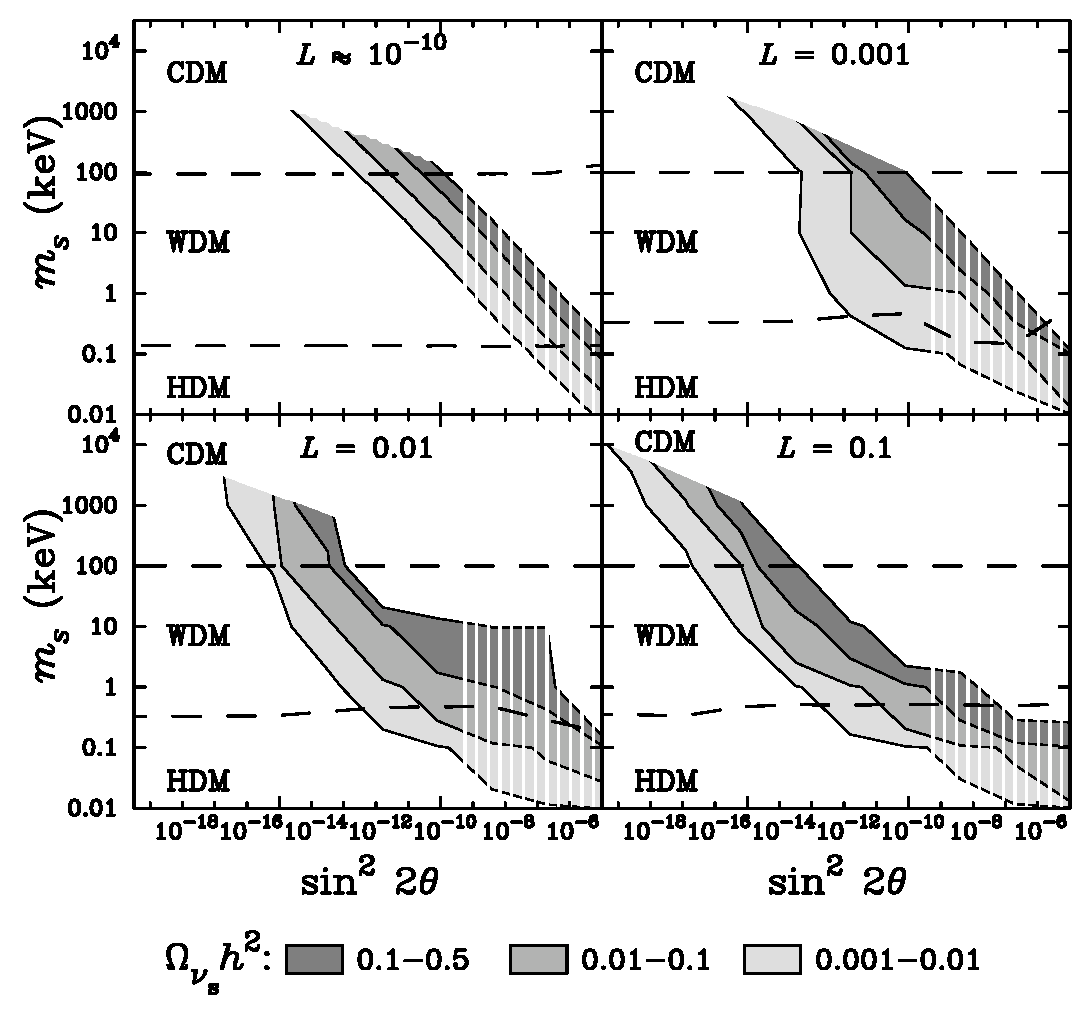
\includegraphics[width=0.9\textwidth]{eps/omegaepanel.eps}
	\caption{Regions of $\Omega_{\nu_s}$ produced by resonant and non-resonant electron neutrino mixing with a sterile neutrino.
	$L$ denotes lepton asymmetry. Regions of parameter space disfavoured by supernova core collapse considerations are shown
	with vertical stripes. From \cite{ref_sterileneutrino}.}
	\label{fig_sterileelectronphase}
	\end{center}
\end{figure}
\begin{figure}[pb]
	\begin{center}
	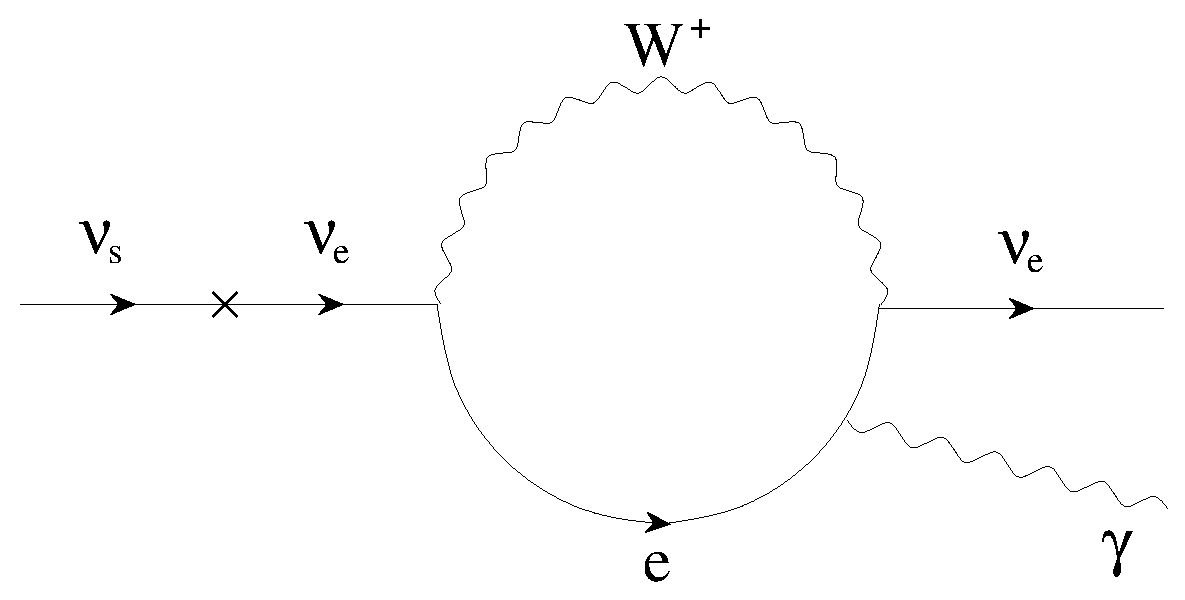
\includegraphics[angle=0,width=0.6\textwidth]{eps/fermiondecay.eps}
	\caption{Feynman diagram for the radiative decay of a sterile neutrino into an active neutrino
	and a photon of energy $\frac{m_{\nu_s}}{2}$.}
	\label{fig_feynmandiag}
	\end{center}
\end{figure}

\subsection{The Fermion Halo}
It has been shown that a non-relativistic self interacting fermion gas may undergo a first order gravitational
phase transition, from a diffuse state to a condensed state \cite{ref_halo2,ref_halo3,ref_halo4}.
Within a Fermi gas, self energy from gravity is balancing with thermal energy. If the gravity dominates, we have a condensed state,
whereas if the thermal energy dominates, we have a diffuse state. The temperature at which the fermions are close to the point of
gravitational collapse is called the critical temperature and is where the phase transition occurs. A simple analytical model has been
proposed by \cite{ref_chavanis}, agreeing quite well with the numerical simulations.

We now briefly discuss the non-relativistic Thomas-Fermi theory for a self gravitating gas of $N$ fermions with mass $m_\nu$ at a
temperature $T$ enclosed in a sphere of radius $R$. For large $N$ we can assume the fermions move in a spherically symmetric mean-field
potential $\phi(r)$ which satisfies Poisson's equations
\begin{eqnarray}
	\frac{d\phi}{dr} &=& \frac{GN}{r^2}
	\label{eqn_halo1} \\
	\frac{dM(r)}{dr} &=& 4\pi r^2 m n
	\label{eqn_halo2}
\end{eqnarray}
The number density ($n$) is determined by the Fermi-Dirac distribution (units $\hbar=c=k=1$)
\begin{equation}
	n=\frac{\rho}{m_\nu}=g_\nu \int \frac{d^3q}{(2\pi)^3} \left[ 1+e^{\left(\frac{q^2}{2 m_\nu T} + \frac{m_\nu \phi}{T}
	- \frac{\mu}{T}\right)}\right]^{-1}
	\label{eqn_halo3}
\end{equation}
For each solution $\phi(r)$ of (\ref{eqn_halo1}), the chemical potential $\mu$ is adjusted so that the constraint
\begin{equation}
	\int^R_0 dr 4\pi r^2 n(r) = N
	\label{eqn_halo4}
\end{equation}
is satisfied. Equations (\ref{eqn_halo2}) and (\ref{eqn_halo3}) are integrated using the boundary conditions
\begin{equation}
	\phi(0)=\phi_0 \qquad \qquad M(0)=0
	\label{eqn_halobounds}
\end{equation}
It is useful to introduce the degeneracy parameter
\begin{equation}
	\eta = \frac{\mu}{T} - \frac{m_\nu \phi}{T}
	\label{eqn_halo5}
\end{equation}
with the strongest degeneracy $\eta_0$ obtained at the centre, fixed by the condition $M(R)=m_\nu N$, where $R$ is the outer boundary.
Outside of $R$, we have the usual $\propto \frac{1}{r}$ Newtonian potential.
Equations (\ref{eqn_halo2}), (\ref{eqn_halo4}) and (\ref{eqn_halo3}) define the gravitational Thomas-Fermi equation, which is solved numerically.

One first solves (\ref{eqn_halo2}) to yield $M(R)$ as a function of $\eta_0$, leaving 3 free parameters:
$N$, $T$ and $R$. $N$ is fixed by setting the fermion mass and using an appropriate total mass consistent with observation.
We make the simple calculation $N=\frac{M}{m_\nu}$.

In \cite{ref_halo}, the values $m_\nu=15$keV, $M=2 \times 10^{12} M_\odot$, $R=200$kpc and $T=3.75 \times 10^{-3}$K were used.
The radius limit is based upon the estimated size of the galaxy halo. The
temperature is estimated as a result of violent relaxation \cite{ref_haloviolentrelax}, and is thus
directly related to the gravitational plus thermal energy.

The solution is a fermion ball (as investigated in this thesis) alongside a low density halo, extending out to the radius $R$.

\subsection{Rotation Curve of Our Galaxy}
Using the numerical mass distribution of the halo, the rotation curve for objects within our galaxy may be calculated. The bulge
and disk must also be included for comparison to data. The total rotation curve for our galaxy is shown
in Figure \ref{fig_halorotation}. The bulge is modelled as a spherically symmetric matter distribution \cite{ref_halobulge} in the form
\begin{equation}
	\rho_b(s)=\frac{e^{-hs}}{2s^3} \int^\infty_0 du \frac{e^{-hsu}}{\left[ (u+1)^8 -1\right]^{\frac{1}{2}}}
	\label{eqn_halobulge}
\end{equation}
where $s=\left( \frac{r}{r_0} \right)^{\frac{1}{4}}$, $r_0$ is the effective radius of the bulge. We adopt values such that
$M_b=1.5\times 10^{10}M_\odot$ \cite{ref_halobulgevalues}.
The contribution of the disk's circular velocity component is modelled as \cite{ref_halodisk}
\begin{equation}
	\Theta_d(r)^2=\Theta_d(r_0)^2\frac{1.97 \left( \frac{r}{r_0}\right)^{1.22}}{\left[\left( \frac{r}{r_0}\right)^2 +0.78^2 \right]^{1.43}}
	\label{eqn_halodisk}
\end{equation}
where we take $r_0=13.5$kpc and $\Theta_d(r_0)=100$km/s. We assume (for simplicity) that the disk does not influence the mass distribution of
either the bulge or the halo.
\begin{figure}[t]
	\begin{center}
	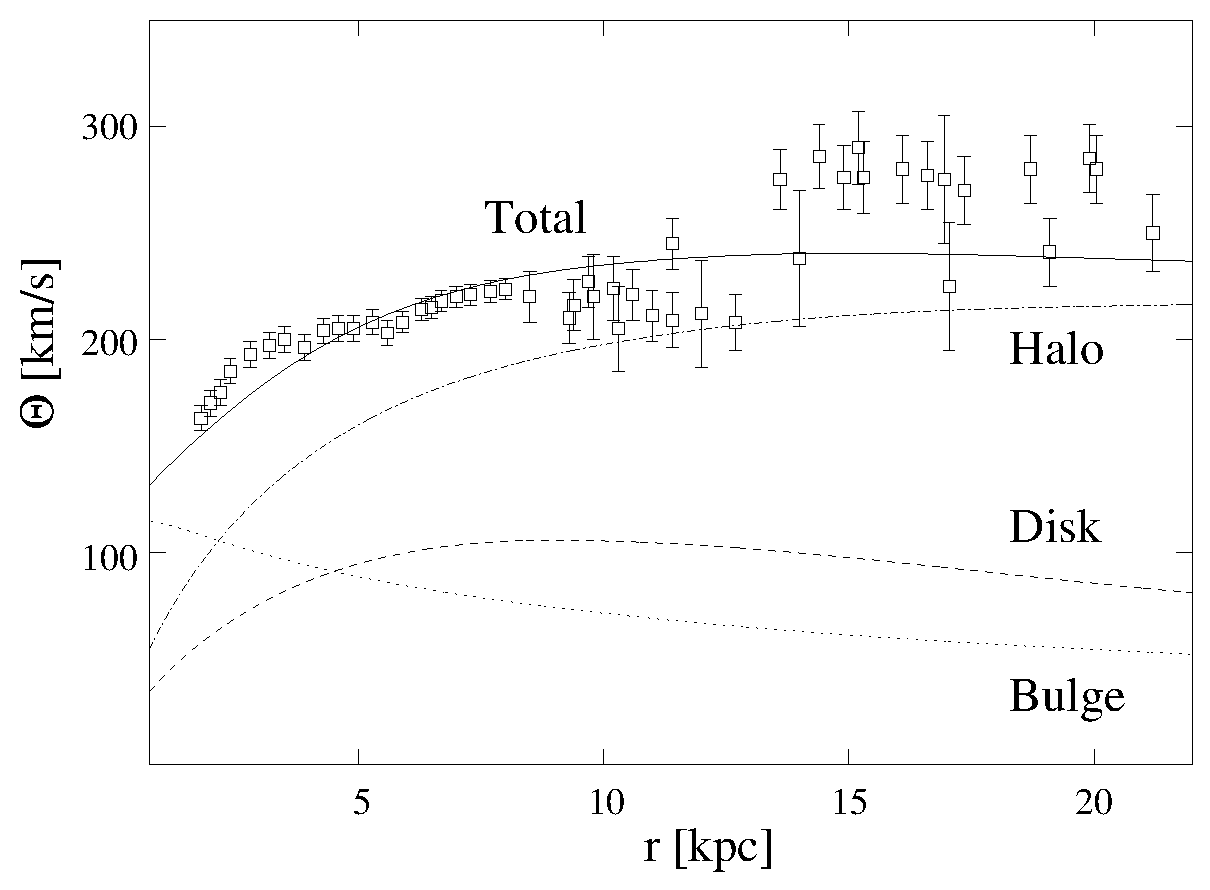
\includegraphics[width=0.9\textwidth]{eps/halo.eps}
	\caption{Fit to the Galactic rotation curve. Data points are from \cite{ref_halodata} and the graph itself is from \cite{ref_halo}.}
	\label{fig_halorotation}
	\end{center}
\end{figure}

The rotation curve clearly shows that the standard disk and bulge models, in combination with the halo theory, describe reasonably the circular
velocity distribution within our galaxy to just beyond a distance of 20kpc. We conclude that the fermion halo sufficiently describes the dark
matter distribution within our own galaxy.

In summary, the Thomas-Fermi theory applied to finite temperature, self gravitating, fermionic gas yields a mass distribution
explaining the dark matter distribution within the Milky Way halo, whilst also producing a fermion ball at the centre. This theory therefore
allows that the fermions in the halo are the same as those at the galactic centre, Sgr A*.
